%
% File acl-hlt2011.tex
%
% Contact: gdzhou@suda.edu.cn
%%
%% Based on the style files for ACL2008 by Joakim Nivre and Noah Smith
%% and that of ACL2010 by Jing-Shin Chang and Philipp Koehn


\documentclass[11pt]{article}
\usepackage{acl-hlt2011}
\usepackage{times}
\usepackage{latexsym}
\usepackage{amsmath}
\usepackage{multirow}
\usepackage{url}
\usepackage{color}
\usepackage[vlined,figure]{algorithm2e}
\usepackage{graphicx} 

\DeclareMathOperator*{\argmax}{arg\,max}

\definecolor{red}{rgb}{1,0,0}

\newcommand{\mnote}[1]{\marginpar{%
  \vskip-\baselineskip
  \raggedright\footnotesize
  \itshape\hrule\smallskip\tiny{#1}\par\smallskip\hrule}}  

\newcommand{\mtodo}[1]{\mnote{\textcolor{red}{#1}}}
\newcommand{\todo}[1]{\textcolor{red}{TODO: #1}}
\newcommand{\secref}[1]{Section~\ref{#1}}
\newcommand{\tabref}[1]{Table~\ref{#1}}
\newcommand{\figref}[1]{Figure~\ref{#1}}
\newcommand{\code}[1]{{\small \tt #1}}
\newcommand{\bm}{\boldsymbol}
\def\bs#1{\boldsymbol{#1}}

\setlength\titlebox{6.5cm}    % Expanding the titlebox

\title{Statistical Machine Translation without Parallel Corpora}

\author{Person\\
  University of Awesome\\
  Location\\
  {\tt person@email}  \And
  Person\\
  University of Awesome\\
  Location\\
  {\tt  person@email}   \And
  Person\\
  University of Awesome\\
  Location\\
  {\tt  person@email}}

\date{}

\begin{document}
\maketitle
\begin{abstract}
\end{abstract}

\section{Introduction} \label{sect:intro}


\section{Related work} \label{sect:relwork}

SMT state of the art: phrase-based \cite{Koehn:2003}, hierarchical \cite{Chiang:2005}, etc.  Will review the phrase-based pipeline in greater detail in \secref{sect:bckg}, and describe our extensions in \secref{sect:mono}. For a recent thorough review of statistical machine translation we refer the reader to \cite{Lopez:2008}.\\

A lot of related work in lexicon induction (e.g. \cite{Rapp:1995,Fung:1998,Koehn:2000,Haghighi:2008,Mimno:2009}).  Although often motivated by the resource constrained machine translation, it was never used in MT.  In this work, we make direct use of these methods in the machine translation pipeline.

\section{Background} \label{sect:bckg}

Review the MT pipeline, emphasizing: phrase scoring and ordering.

\section{Reducing the Parallel Data requirement / Estimating Parameters from Monolingual Data} \label{sect:mono}

\subsection{Phrase extraction}  \label{sect:extract}

Building on the many successful efforts in bilingual lexicon induction from monolingual corpora, we compile a table of {\it phrasal} translations from monolingual corpora. Current methods for inducing a bilingual lexicon, or, equivalently, a unigram phrase translation table, are computationally expensive as each source and target word pair must be scored. That is, the models must  compute $|V_s| * |V_t|$ similarity scores, where $|V_s|$ and $|V_t|$ are the sizes of the source and target vocabularies, respectively. As we search for longer phrase pairs, this search space increases exponentially with the size of the  {\it n}-grams. Exhaustively scoring all phrase pairs up to length three requires $|V_s|^3 * |V_t|^3 $ score computations. We prune the phrase pair search space using methods from Information Retrieval, like that used in \newcite{Uszkoreit:2010}. 

First, we compose a set of all {\it n}-grams up to length three in the source side monolingual corpus and in the target side monolingual corpus. We store each source side {\it n}-gram's frequency along with the phrase. We also store each target side {\it n}-gram in a frequency inverted index. We index target side phrases by frequencies within a band of their actual observed frequency in the monolingual corpus. Additionally, for the target side {\it n}-grams, we look up each word in the phrase in our bilingual dictionary, and we store a set of source side words that translate into any word in the phrase. \mtodo{discuss dictionary(ies)}

These sets of observed phrases, frequencies, and the bilingual dictionary together allow us to effectively filter our search space using combinations of inverted indices. Given a source side test set, we collect  {\it n}-grams up to length three (in our Urdu test set, there are 36,423 phrases), as we did for the monolingual corpora. We then look up each source side phrase's monolingual corpus frequency and consult the target side inverted index to find a list of target side phrases that occur in the same frequency band. Of those target side phrases, we keep only the ones with at least one \mtodo{discuss dictionary parameters} word translating into a word in the source side phrase. 

This method of pruning the phrase pair search space involves two manually tuned parameters. In order to evaluate the filtered phrase tables and tune the parameters, we used the Moses decoder's trace function to find the set of phrases used in decoding an Urdu test set. \mtodo{data details?} We compare our filtered phrase tables to this set of phrase translation rules and attempt to maintain as many of them as possible, while pruning the set of phrase pairs down to manageable size. 

Our baseline phrase table is generated using a bilingual dictionary. For each Urdu test set phrase up to length three, we generated English phrases from all combinations of dictionary translations and all possible reorderings. For the baseline and our pruning methods, the number of filtered phrase pairs and the percent of phrases used by the Moses decoder not pruned away are given in Table \ref{table:prune}.  

\begin{table*}
\small
\begin{center}
\label{table:prune}
\begin{tabular}{|c|c|c|c|c|}
\hline
Pruning filters & Phrase Pairs & Percent of total search space & Findable types & Findable tokens \\
\hline
Unpruned phrase table & 37,322,465,985 & 100\% & 100\% & 100\% \\
Baseline phrase pairs & 29245036 & 0.08\% & 15.37 & 25.07 \\
Frequency-based pruning & 4,450,429,494 & 11.92\% & 85.21\% & 87.48\% \\
Frequency and Dictionary pruning & 1,436,823,109 & 3.85\% & 57.79\% & 58.76\% \\
\hline
\end{tabular}
\caption{This shows the tradeoff between pruning the phrase pair search space and the accuracy of the final set of phrase pairs. The findable types and tokens measures refer to the percent of phrase types and tokens used by Moses to decode a test set that are not pruned away.}
\end{center}
\end{table*}


Second round of pruning: after monolingual feature extraction, before re-ordering estimation. Needs to be discussed after explanation of those methods? 

\subsection{Phrase scoring} \label{sect:score}

In place of phrase translation probabilities estimated from bilingual alignments, we propose to compute similarity scores computed (almost) solely from monolingual resources.\\

\noindent\emph{Contextual similarity}.  We extend the vector space approach of \cite{Rapp:1999} to compute similarity between \emph{phrases} in source and target language.  More formally, assume that $(f_{1}, f_{2}, \dots f_{N})$ and $(e_{1}, e_{2}, \dots e_{M})$ are (arbitrarily indexed) source and target vocabularies, respectively.  A source phrase $f$ (target phrase $e$) is represented with an $N$ ($M$) dimensional vector.  Only the components corresponding to words that appear in the context of $f$ ($e$) in data take on non-zero values, which typically measure how ``unique'' a word is to the context in the dataset.  Next, $f$'s contextual vector is projected by mapping each component to a component in the target space corresponding to its translation (taken from a small seed dictionary), but retaining the source component value.  Finally, the pair ($f, e$) is scored by computing similarity between the (projected) source and target vectors.  Various means of computing the component values and vector similarity measures have been proposed in literature (e.g. \cite{Rapp:1999,Fung:1998}).  While the quality of the resulting induced lexicon depends on the data, we found the following to work best in our experiments.  We compute the value of the $k$-th component of $f$'s contextual vector  as follows: 

\begin{equation*}
w_{k}^{(i)} = n_{i,k} \times (log( {n / n_{i}}) + 1)
\end{equation*}

\noindent where $n_{i,k}$ and $f_{k}$ are the number of times $f_{k}$ appears in the context of $f_{i}$ and in the entire corpus, and $n$ is the maximum number of occurrences of any word in the data.  Intuitively, the more frequently $f_{k}$ appears with $f_{i}$ and the less common it is in the corpus in general, the higher its component value.  Similarity between two resulting vectors is measured as a cosine of the angle between them.\\

\noindent\emph{Temporal similarity}. Online content is often published along with temporal information: news feeds, for example, are comprised of news stories annotated with date and time of publication.  The feeds are specialized for the target geographical locations and vary in content across languages.  Still, many events are deemed relevant to multiple audiences and the news stories related to them appear in several languages, although rarely as direct translations of one another.  Phrases associated with these events will appear with increased frequency in multiple languages around the dates when these events are reported.  Such weak synchronicity provides a cue about the relatedness of phrases across the two languages.  In order to score a pair of phrases across languages, we can compute the similarity of their temporal signatures. To generate a time sequence for a given word, we first sort the set of (time-stamped) documents of our corpus into a sequence of equally sized temporal bins.  We then count the number of occurrences of a phrase in each bin.  Changing the size of the bin or computing counts in a sliding window instead can recover some accuracy if the temporal alignment between two languages in our dataset is poor \cite{Klementiev:2006b}.  Finally, we normalize the sequence and use either the cosine measure to score similarity. \\

\noindent\emph{Orthographic / phonetic similarity.} Etymologically related words often retain similar spelling across languages with the same writing system, and the edit distance can be used to measure their orthographic similarity.  We extend this idea to phrases by using word alignments within a phrase pair (see \secref{sect:extract}): we score pairs of aligned words and normalize by their average length. \mtodo{Make sure it is correct.}

We can further extend this idea to language pairs not sharing the same writing system, since many cognates and transliterated words are phonetically similar.  Following \cite{Virga:2003,Irvine:2010a}, we treat transliteration as a monotone character translation task and use a generative model\mtodo{Argue that enough training data is easy to get} to propose a transliteration of tokens in a source phrase.  Once the source words are mapped to the target writing system, the phrase similarity is computed as before.\\

Depending on the available monolingual data (and its associated metadata), various other similarity scores can be computed and added to the list (see, e.g. \cite{Schafer:2002}).

\subsection{Reordering} \label{sect:order}

\begin{figure}[ht]
\vskip 0.1in
\begin{center}
\centerline{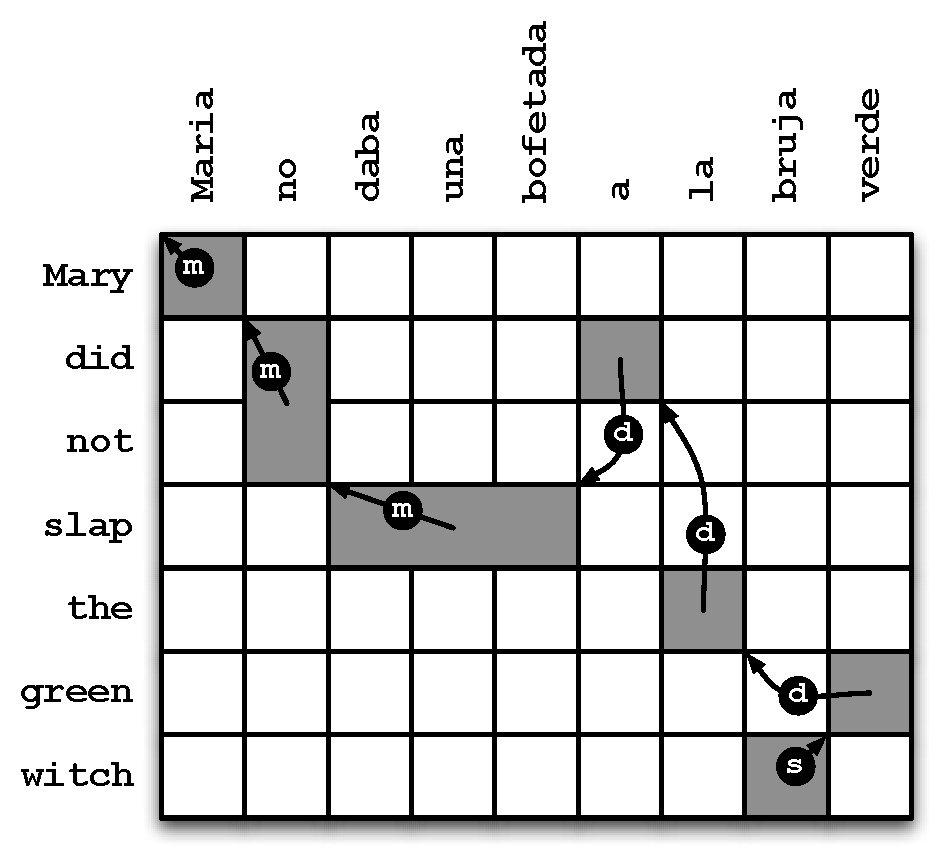
\includegraphics[scale=0.5]{../figures/reorderfeats/reorderfeats.pdf}} %[width=\columnwidth]
\caption{Example alignment along with three kinds of orientations: monotone (m), swap (s), and discontinuous (d). }
\label{fig:reorderfeats}
\end{center}
%\vskip -0.2in
\end{figure}

Describe the algorithm for estimating orientation probabilities.  Talk about the issue of too much weight on out-of-order orientation.  Talk about where $w$ comes from.  Mention that it is not as expensive as it looks.  The intuition is simple - see if translated phrases tend to keep the order.

 \footnote{$\#_{S}(x)$ returns the count of object x in multiset S.}

\SetAlFnt{\relsize{-1.5}}

\begin{algorithm}[t]

 \SetKwFunction{CollectOccurs}{CollectOccurs}
 \SetKwBlock{Body}{}{}
 \SetCommentSty{text}
 \SetFuncSty{text}

 \hrule \vskip 0.2cm

  \KwIn{Source and target phrases $f$ and $e$, source and target corpora $\emph{C}_f$ and $\emph{C}_e$, phrase table pairs $\emph{T} = \{(f^{(i)}, e^{(i)})\}_{i=1}^{N}$.}
  \KwOut{Orientation features $(p_m, p_s, p_d)$.}
  
  \vskip 0.2cm \hrule \vskip 0.2cm

  $S_f \leftarrow$ sentences containing $f$ in $\emph{C}_f$\;
  $S_e \leftarrow$ sentences containing $e$ in $\emph{C}_e$\;
  
  $(B_f, -, -) \leftarrow \CollectOccurs(f, \cup_{i=1}^{N} f^{(i)}, S_f)$\;
  $(B_e, A_e, D_e) \leftarrow \CollectOccurs(e, \cup_{i=1}^{N} e^{(i)}, S_e)$\;
    
  $c_m = c_s = c_d = 0$\;
  
  \vskip 0.1cm 

  \ForEach{$f_b \in B_f$} {
    \ForEach{translation $e^{*}$ of $f_b$ in $\emph{T}$} {

      $c_m = c_m + \#_{B_e}(e^{*})$\; 
       $c_s = c_s + \#_{A_e}(e^{*})$\; 
       $c_d = c_d + \#_{D_e}(e^{*})$\; 
    }
  }
  
  $c \leftarrow c_m + c_s + c_d$;
    
  \Return{$({c_m \over c}, {c_s \over c}, {c_d \over c})$}

  \vskip 0.2cm \hrule \vskip 0.2cm

  \CollectOccurs{$r$, $R$, $S$} \Body{
   $B \leftarrow ()$; $A \leftarrow ()$; $D \leftarrow ()$\;

    \ForEach{sentence $s \in S$} {
      \ForEach{occurrence of phrase $r$ in $s$} {
        $B \leftarrow B$ + $($longest preceding and in $R)$\;
        $A \leftarrow A$ + $($longest following and in $R)$\;
        $D \leftarrow D$ + $($longest discontinuous and in $R)$\;
      }
    }
    
    \Return{($B$, $A$, $D$)}\;
  }
  
  \vskip 0.2cm \hrule \vskip 0.2cm

  \caption{Estimating reordering probabilities from monolingual data.} \label{fig:reorder}
  %\vskip -0.2in
\end{algorithm}

\section{Experiments} \label{sect:exp}

\subsection{Data}
Describe data we use in the experiments:  Europarl \cite{Koehn:2005}, Gigaword, our own crawls\footnote{Promise to distribute after publication.}.

\subsection{Single language}

\begin{enumerate}
\item {\em Phrase features}.  (a) Augment phrase scores with mono features.  If we see better performance, reduce the amount of parallel data until it matches the performance of the original system.  Make the tradeoff argument.  (b) ({\bf lesion experiments}) See how well we do with mono features alone.
\item {\em Orientation features}. Use mono orientation features.
\item {\em Induce phrase table}.
\item {\em Put everything together}.  Run the entire pipeline.
\end{enumerate}

\subsection{Big experiment}

Now, run the entire pipeline on a handful of languages extracting monolingual features from the Gigaword and our crawls.

\section{Discussion} \label{sect:disc}

\section{Conclusions and Future Work} \label{sect:conc}

First to make use of plentiful monolingual data to reduce the dependence on expensive parallel data.  In particular:

\begin{itemize}
\item Showed that augmenting standard pipeline with monolingual features helps.
\item Demonstrated that monolingual features are informative enough on their own for a competitive system.
\item Proposed an algorithm for estimating orientation probabilities from monolingual data alone.
\item Build complete systems for X low-resource languages.
\end{itemize}

%\section*{Acknowledgments}
%The authors would like each other and their parents.

\bibliographystyle{acl}
% you bib file should really go here 
\bibliography{lowresmt}

\end{document}
